%%%%%%%%%%%%%%%%%%%%%%%%%%%%%%%%%%%%%%%%%%%%%
%   Copyright (c) 2008 Anne-Lise Caillat, Christophe Dutang, 					     %
%	V\'eronique Larrieu and Triet Nguyen                                                                                    %       
%                                                                                                                                                       %
%    This program is free software; you can redistribute it and/or modify                               %
%    it under the terms of the GNU General Public License as published by                         %
%    the Free Software Foundation; either version 2 of the License, or                                   %
%    (at your option) any later version.                                                                                          %
%                                                                                                                                                        %
%    This program is distributed in the hope that it will be useful,                                             %
%    but WITHOUT ANY WARRANTY; without even the implied warranty of                        %
%    MERCHANTABILITY or FITNESS FOR A PARTICULAR PURPOSE.  See the          %         
%    GNU General Public License for more details.                                                                    %
%                                                                                                                                                         %
%    You should have received a copy of the GNU General Public License                           %
%    along with this program; if not, write to the                                                                            %
%    Free Software Foundation, Inc.,                                                                                             %
%    59 Temple Place, Suite 330, Boston, MA 02111-1307, USA                                            %
%                                                                                                                                                         %
%%%%%%%%%%%%%%%%%%%%%%%%%%%%%%%%%%%%%%%%%%%%%%
%%% ----- File part of R package gumbel -----
%%%
%%%			Sweave vignette file
%%% 

\documentclass[11pt]{article}

%\VignetteIndexEntry{Key characteristics of the Gumbel copula [in French]}
%\VignettePackage{gumbel}


%symbole math de l'American Mathematical Society (AMS)
\usepackage{amsfonts,amssymb,amsmath}
%utiliser les regles de typographie francaise
\usepackage[frenchb]{babel}
%encodage des accents selon la norme UNIX
\usepackage[utf8]{inputenc}
%pour les en tetes
\usepackage{fancyhdr}
\usepackage{fancyvrb}
\usepackage{fancybox}
\pagestyle{headings}
%pour la mise en page


% layout sinon utiliser vmargin
\normalsize\setlength{\parskip}{\baselineskip}
\setlength{\oddsidemargin}{20mm}
\setlength{\evensidemargin}{20mm}
\setlength{\voffset}{-1in}
\setlength{\hoffset}{-1in}
\setlength{\textwidth}{175mm}
\setlength{\topmargin}{05mm}
\setlength{\headheight}{10mm}
\setlength{\headsep}{10mm}
\setlength{\topskip}{0mm}
\setlength{\textheight}{240mm}

%citation
\usepackage{natbib}
%note de bas de page
\usepackage[stable]{footmisc}
%graphique
\usepackage[dvips]{graphicx}
\usepackage{color,graphics}


\newcommand{\pkg}{\textbf}
\newcommand{\sigle}{\textsc}
\newcommand{\code}{\texttt}
\newcommand{\soft}{\textsf}
\newcommand{\txtm}[1]{\textrm{~~#1~~}}
\newcommand{\expo}{\textsuperscript}

\usepackage{Sweave}
\begin{document}
\Sconcordance{concordance:gumbel.tex:gumbel.Rnw:%
1 69 1 1 0 637 1}


\thispagestyle{empty}
 
\vspace{10cm}
\begin{center} {\huge \textbf{COPULE DE GUMBEL}} \end{center}
\vspace{5cm}
\begin{center} {\Large Caillat Anne-lise, Dutang Christophe,} \end{center}

\begin{center} {\Large Larrieu Marie V\'eronique et NGuyen Triet} \end{center}

\vspace{2cm}
\begin{center} {\large Groupe de travail ISFA 3} \end{center}

\begin{center} {\large sous la direction de St\'ephane Loisel} \end{center}
\vspace{1cm}
\begin{center} {\large Ann\'ee Universitaire 2007-2008} \end{center}


\newpage


\tableofcontents

\newpage

\section{Introduction}

Les copules constituent un outil statistique permettant de mod\'eliser la d\'e\-pen\-dance 
entre des variables al\'eatoires. La fonction copule relie en effet la densit\'e jointe aux 
densit\'es marginales et contient ainsi toute l'information sur la structure de d\'ependance du mod\`ele.

\medskip

Nous nous int\'eresserons dans ce document \`a une copule particuli\`ere, soit la copule de 
Gumbel. Dans la litt\'erature, elle est parfois appel\'ee copule de Gumbel - Hougaard. Pour la 
clart\'e de l'expos\'e, nous traiterons ici le cas bivari\'e et nous finirons par une g\'en\'eralisation 
au cas multivari\'e. La plupart des informations sont tir\'ees de \cite{nelsen}.

\medskip

Ce document s'articulera principalement autour de quatre axes : nous d\'e\-finirons tout d'abord la 
copule de Gumbel ainsi que ses caract\'eristiques, nous pr\'esenterons ensuite les techniques 
de simulation. Puis nous pr\'esenterons l'impl\'ementation des divers outils pr\'esent\'es jusqu'ici, ainsi
que les m\'ethodes de calibration. Enfin, nous termirons par une application de la copule de Gumbel
au produit indiciel.

\section{Caract\'eristiques}

\subsection{D\'efinition}

La copule de Gumbel est d\'efinie par la fonction bivari\'ee :

$$C_\alpha\left(u,v\right)=\exp\left[-\left(\left(-\ln u\right)^\alpha+\left(-\ln v\right)^\alpha\right)^{\frac{1}{\alpha}}\right],$$

o\`u $\alpha\geq1$ est le param\`etre de la copule.

\subsection{Copule archim\'edienne}
Si on prend $\phi_\alpha(t)=\left(-\ln t\right)^\alpha$ avec $\alpha\geq1$ et $t\in [0,1]$ comme fonction g\'en\'eratrice, on v\'erifie facilement que :

\begin{itemize}
\item[]
\item[$\bullet$] la fonction g\'en\'eratrice inverse est $\phi_\alpha^{-1}(t)=e^{-t^{1/\alpha}}$,
\item[]
\item[$\bullet$] $\phi_\alpha(0)=+\infty$, ce qui traduit le caract\`ere strict du g\'en\'erateur
\item[]
\item[$\bullet$] $\phi_\alpha(1)=0$,
\item[]
\item[$\bullet$] $\phi_\alpha^\prime(t)=-\frac{\alpha}{t}(-\ln t)^{\alpha-1}$ et $\phi_\alpha^\prime(t)<0$ pour $\alpha\geq1$,
\item[]
\item[$\bullet$] $\phi_\alpha^{\prime\prime}(t)=\frac{\alpha}{t^2}(-\ln t)^{\alpha-2}\left[\alpha-1-\ln t\right]$ et $\phi_\alpha^{\prime\prime}(t)\geq0$ pour $\alpha\geq1$.
\item[]
\end{itemize}
Ainsi, $\phi$ est une fonction continue strictement d\'ecroissante de $[0,1]$ dans $[0,+\infty]$, convexe et est un
g\'en\'erateur strict.

Et nous retrouvons la famille de Gumbel par la relation $\phi_\alpha^{-1}\left(\phi_\alpha(u)+\phi_\alpha(v)\right)$.
Les copules archim\'ediennes forment des familles de copules qui poss\`edent plusieurs propri\'et\'es 
int\'eressantes\footnote{Certaines de ces propri\'et\'es seront utilis\'ees dans les paragraphes qui 
suivent afin de mettre l'accent sur certaines carac\-t\'e\-ristiques propres \`a la copule de Gumbel.}. 

\subsection{Fonction de r\'epartition}
La fonction copule $C_\alpha$ est par d\'efinition la fonction de r\'epartition d'un couple de variables al\'eatoires \`a marginales uniformes et de loi jointe $C_\alpha$.
\begin{center}
\fbox{$
\forall \alpha \geq 1, \forall (u,v) \in [0,1]^2,~C_\alpha\left(u,v\right)=\exp\left[-\left(\left(-\ln u\right)^\alpha+\left(-\ln v\right)^\alpha\right)^{\frac{1}{\alpha}}\right].
$}
\end{center}


\subsection{Densit\'e}
Nous savons que la densit\'e d'une copule archim\'edienne, de g\'en\'erateur $\phi$ deux fois diff\'erentiable, est telle que
$$c_\alpha(u,v)=-\frac{ \phi_{\alpha}^\prime\left(C_\alpha(u,v)\right) \phi_{\alpha}^\prime(u) \phi_{\alpha}^\prime(v)}{ \phi_{\alpha}^\prime\left(C_\alpha(u,v)\right)^3}$$

Donc
\begin{footnotesize}
$$c_\alpha(u,v)=-\frac{\frac{\alpha}{C_\alpha(u,v)^2}\left[\left(-\ln u\right)^\alpha+\left(-\ln v\right)^\alpha\right]^\frac{\alpha-2}{\alpha}   \left[\alpha-1+\left[\left(-\ln u\right)^\alpha+\left(-\ln v\right)^\alpha\right]^\frac{1}{\alpha}\right]   \frac{-\alpha}{u}\left(-\ln u\right)^{\alpha-1}\frac{-\alpha}{v}\left(-\ln v\right)^{\alpha-1}}{-\frac{\alpha^3}{C_\alpha(u,v)^3}\left[\left(-\ln u\right)^\alpha+\left(-\ln v\right)^\alpha\right]^{3\left(\frac{\alpha-1}{\alpha}\right)}}$$
\end{footnotesize}

Nous obtenons la densit\'e suivante :
\begin{center}
\fbox{$\forall u, v \in ]0,1[^2, c_\alpha(u,v)=C_\alpha(u,v) \left[ \phi_{\alpha}(u)+\phi_{\alpha}(u)  \right]^{\frac{1}{\alpha}-2}  \left[ \alpha-1+\left( \phi_{\alpha}(u)+\phi_{\alpha}(u)\right)^{\frac{1}{\alpha}} \right] \frac{\phi_{\alpha-1}(u)\phi_{\alpha-1}(v)}{uv}.
$}
\end{center}
L'expression supra de la densit\'e n'est pas valable sur les bords du pav\'e $[0,1]\times [0,1]$. Sur les bords du domaine, nous avons les expressions suivantes :
$$
\forall u>0,v<1, c_\alpha(u,0)=c_\alpha(0,u) = c_\alpha(1,v) =c_\alpha(v,1)=0,
$$
tout en sachant que la densit\'e n'est pas d\'efinie aux points $(0,0)$ et $(1,1)$\footnote{cf annexe \ref{densiteDemo}.}.

\medskip

La copule de Gumbel est caract\'eris\'ee par des concentrations importantes dans les queues de distribution\footnote{on a $c_\alpha(0,0)=c_\alpha(1,1)``=``+\infty$.}. 
Sur la figure \ref{densite}, on constate que la copule de Gumbel est dissym\'etrique \`a droite. Ce r\'esultat se retrouve dans les coefficients de
d\'ependance de queue dans la section \ref{dependance}. 

% \begin{figure}[!htb]
% \begin{center}
% 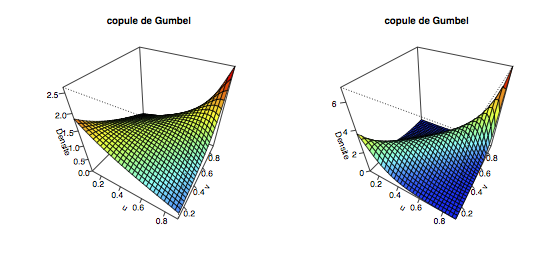
\includegraphics[scale=0.6]{img/densite}
% \caption{Densit\'e de la copule de Gumbel ($\alpha=1,5$ \`a gauche et $\alpha=3$ \`a droite)}
% \label{densite}
% \end{center}
% \end {figure}


\subsection{Copule singuli\`ere}

Comme la fonction copule $C_\alpha$ est deux fois diff\'erentiable par rapport \`a $u$ et $v$, alors la copule de Gumbel ne poss\`ede pas de partie singuli\`ere.

\subsection{Valeur particuli\`ere du param\`etre $\alpha$}

Les diff\'erents d\'ependances limites sont r\'esum\'ees dans le tableau infra \ref{parametre}. 
Les d\'emonstrations se trouvent en annexe \ref{parametreDemo}.
\begin{table}[!htb]
\center
\begin{tabular}{lccc}
\hline
$\alpha$ & $1$ & $]1,+\infty[$ & $+\infty$\\
\hline
$C_\alpha$ & $C^\bot$ & $C_\alpha$ & $C^+$\\
\hline
type & Ind\'ependance & D\'ependance positive & Comonotonie\\
\hline
\end {tabular}
\caption{Valeur particuli\`ere de $\alpha$}
\label{parametre}
\end{table}

La valeur au risque ou ``Value at Risk'' \'etant comonotone additive, on retrouve le fait que la VaR de la somme
est la somme des VaR lorsque les variables sont comonotones. On consid\`ere un couple al\'eatoire structur\'e
par $C_\alpha$ et de marginales normales centr\'ees r\'eduites. Sur la figure \ref{var90somme}, nous avons trac\'e la VaR
\`a 90\% de la variable $X+Y$ en fonction du param\`etre $\alpha$ de la copule, o\`u $X$ et $Y$
sont de loi normale centr\'ee r\'eduite. On constate que $VaR(X+Y)$ tends
vers $VaR(X)+VaR(Y)$. Le caract\`ere \'eratique vient du fait que la VaR est calcul\'ee par simulation\footnote{\`a l'aide 
de la fonction \code{quantile} ou de la fonction \code{VaR} du package \pkg{actuar}. } (comme le 90\expo{\`eme}
percentile du vecteur simul\'ee).



\subsection{Mesures de d\'ependance}
Il y a maintes fa\c{c}ons de mesurer la d\'ependance entre deux variables al\'eatoires. Nous pr\'esentons ici le tau de Kendall
et le rho de Spearman, deux mesures de concordance classiques. 

\subsubsection{Coefficient de corr\'elation de Kendall}
Le tau de Kendall est d\'efini par
$$\tau \stackrel{\triangle}{=} 4\int\!\!\!\!\int_{[0,1]^2}C(u,v)dC(u,v)-1 = 4 E\left(C\left(U,V\right)\right)-1=4 E(X)-1.$$
o\`u $U$ et $V$ sont deux variables al\'eatoires uniformes et $X$ la variable al\'eatoire $C_\alpha(U,V)$.
Pour une copule archim\'edienne, la fonction de r\'epartition de $X$ est donn\'ee par

$$K_C(t)=t-\frac{\phi_\alpha(t)}{\phi_\alpha^\prime(t)}$$

soit dans le cas de la copule de Gumbel, 
$$K_C(t)=t-\frac{t\ln t}{\alpha}$$

Ainsi, la densit\'e de $X$ 
$$K_C^\prime(t)=1-\frac{1}{\alpha}-\frac{\ln t}{\alpha}.$$
Par cons\'equent, on a 
\begin{align*}
 E(X) &= \int^1_0tK_C^\prime(t)dt= \left[\frac{t^2}{2}\left(1-\frac{1}{\alpha}\right)\right]^1_0-\int^1_0\frac{t\ln t}{\alpha}dt \\
      &= \frac{1}{\alpha}\left(1-\frac{1}{\alpha}\right) - \frac{1}{\alpha}\left(\left[\frac{t^2}{2}\ln t\right]^1_0-\left[\frac{t^2}{4}\right]^1_0\right)
      =\frac{1}{2}\left(1-\frac{1}{2\alpha}\right)\\
\end{align*}

D'o\`u le tau de Kendall s'exprime de la mani\`ere suivante :
\begin{center}
\fbox{$\tau = \frac{\alpha-1}{\alpha}.$}
\end{center}

\medskip

Le param\`etre $\alpha$ mesure le degr\'e de d\'ependance entre les risques. Plus il est \'elev\'e, plus la d\'ependance est forte. 
On retrouve le fait que $C_{\infty}=C^+$, puisque le tau de Kendall tend vers 1.



\subsubsection{Coefficient de corr\'elation de Spearman}

Le $\rho$ de Spearman quant \`a lui se d\'efinit par

$$\rho_S = 12\int\!\!\!\!\int_{[0,1]^2}C(u,v)dudv-3$$

Cependant, il n'y a pas de formules explicites pour le $\rho$ de Spearman dans le cas de la copule de Gumbel.

\subsection{D\'ependance des queues et copule extr\^eme}
\label{dependance}
Le concept de d\'ependance de queue renseigne sur la ``quantit\'e'' de d\'e\-pen\-dance 
au niveau des queues de distribution. C'est un outil pertinent pour l'\'etude de la survenance simultan\'ee de valeurs extr\^emes.
C'est une mesure locale contrairement au tau de Kendall et au rho de Spearman qui mesure la d\'ependance sur l'ensemble de la distribution.
On d\'efinit les coefficients de d\'ependance de queue \`a gauche et \`a droite pour un couple $(X,Y)$ par
$$
\lambda_L = \underset{t\rightarrow0^+}{\lim} P(Y > F_Y^{-1}(t) / X > F_X^{-1}(t)) \txtm{et} \lambda_U = \underset{t\rightarrow1^-}{\lim} P(Y > F_Y^{-1}(t) / X > F_X^{-1}(t)).
$$

\medskip
Pour la copule de Gumbel, il existe des formules explicites pour $\lambda_U$ et $\lambda_L$.
\begin{center}
\fbox{$ \lambda_L = 0 \txtm{et} \lambda_U = 2-2^{\frac{1}{\alpha}}. $}
\end{center}
On retrouve le fait que la copule est asym\'etrique \`a droite.

\medskip


La copule de Gumbel est une copule extr\^eme car elle v\'erifie la propri\'et\'e du 
max-stabilit\'e\footnote{c'est la seule copule archim\'edienne v\'erifiant cette propri\'et\'e, cf. annexe \ref{extreme}.} 
$$
C_\alpha\left(u^{\frac{1}{n}},v^{\frac{1}{n}}\right)^n = C_\alpha(u,v).
$$
La propri\'et\'e de max-stabilit\'e s'interpr\`ete de la mani\`ere suivante. Soient deux vecteurs
al\'eatoires $(X_1,\dots,X_n)$ et $(Y_1,\dots,Y_n)$ identiquement distribu\'es tels que 
les couples $(X_j, Y_j)$ ont la mÍme copule $C$. \\
On pose $C_{max}$ la copule du couple 
$(X_{(n)},Y_{(n)}) = (\underset{1\leq i\leq n}{\max}(X_i), \underset{1\leq i\leq n}{\max}(Y_i))$.
Par \cite{nelsen2}, nous obtenons la propri\'et\'e suivante :
$$
C_{max} = C\left(u^{\frac{1}{n}},v^{\frac{1}{n}}\right)^n.
$$
Autrement dit pour la copule de Gumbel, le couple $(X_j, Y_j)$ et le couple 
$(X_{(n)},Y_{(n)})$ ont la mÍme copule.



\subsection{Copule multivari\'ee}

On sait que pour les copules archim\'ediennes la propri\'et\'e de super modularit\'e en dimensions $n$ est 
\'equivalent \`a ce que le g\'en\'erateur $\phi$ soit compl\`etement monotone (i.e. $\forall i,~(-1)^i \frac{d^i\phi(t)}{dt^i}\geq 0$ ).
D'apr\`es \cite{nelsen}, le g\'en\'erateur de la copule de Gumbel est compl\`etement monotone. Par
cons\'equent, la copule de Gumbel multivari\'ee se d\'efinit de la mani\`ere suivante
\begin{center}
\fbox{$C_\alpha\left(u_1,\dots,u_n\right)=\exp\left(-\left[\sum\limits_{i=1}^n\left(-\ln u_i\right)^\alpha\right]^{1/\alpha}\right)$}
\end{center}

\medskip

Pour une copule archim\'edienne, la densit\'e s'exprime de la mani\`ere suivante
$$
c(u_1,\dots, u_n) = \left(\phi^{-1}\right)^{(n)}( \phi(u_1)+\dots + \phi(u_n)) \prod_{i=1}^n \phi'(u_i)
$$
d'apr\`es \cite{savutrede}. Malheureusement pour la copule de Gumbel, la d\'eriv\'ee
$n$\expo{i\`eme} de l'inverse du g\'en\'erateur n'a pas d'expressions explicites. Pour $n=3$, nous obtenons
$$
c_\alpha(u_1,u_2,u_3) = C_\alpha(u_1,u_2,u_3) \frac{ \phi_{\alpha-1}(u_1)\phi_{\alpha-1}(u_2)\phi_{\alpha-1}(u_3) }{u_1u_2u_3} 
\Sigma^{\frac{1}{\alpha}-3} \left[ (2\alpha-1)(\alpha-1) + 3(\alpha-1)\Sigma^{\frac{1}{\alpha}}+\Sigma^{\frac{2}{\alpha}} \right],
$$
o\`u $\Sigma$ est d\'efini par $\phi(u_1)+\phi(u_2)+\phi(u_3)$. 




\section{Simulation}

Il existe plusieurs algorithmes pour simuler des variables al\'eatoires selon une copule bien pr\'ecise. Les deux algorithmes infra sont sp\'ecifiques aux copules archim\'ediennes. 

\subsection{Algorithme ``$K_C$''}

D'apr\`es \cite{nelsen2}, le couple de variables al\'eatoires $\left(C_\alpha(U,V), \frac{\phi_\alpha(U)}{\phi_\alpha(U)+\phi_\alpha(V)}\right)$ est \`a composantes ind\'ependantes. Par cons\'equent, on en d\'eduit l'algorithme suivant
\begin{enumerate}
\item simuler $(y,t) \stackrel{iid}{\sim} \mathcal U(0,1)$
\item $x:=K_C^{-1}(t)$ o\`u $K_C(t)=t-\frac{t\ln t}{\alpha}$
\item $u := \phi^{-1}\left(\phi(x)y \right)$ et $v := \phi^{-1}\left(\phi(x)(1-y) \right)$
\end{enumerate}
La non g\'en\'eralisation en dimension $n$ et la non existence de formule explicite pour $K_C^{-1}$ nous ont incit\'e \`a chercher un autre algorithme plus puissant.

\subsection[Repr\'esentation \`a facteurs communs]{Repr\'esentation \`a facteurs communs de \cite{marshall}}
L'approche de \cite{marshall} consiste \`a utiliser une variable al\'eatoire $\Theta$ pour un vecteur al\'eatoire $(X_1, \dots, X_d)$ tel que les composantes $X_i$ sont ind\'ependantes conditionnellement \`a $\Theta$. La loi jointe du vecteur $(X_1, \dots, X_d)$ est donn\'ee par
$$
F_{X_1, \dots, X_d}(x_1, \dots, x_d)=L_\Theta\left( \sum_{i=1}^d L^{-1}_\Theta\left(F_{X_i}(x_i)\right) \right)
$$
o\`u $L_\Theta$ d\'esigne la transform\'ee de Laplace de la variable al\'eatoire $\Theta$. De plus, l'algorithme suivant permet de simuler des variables al\'eatoires de copule archim\'edienne $L^{-1}_\Theta$ :
\begin{enumerate}
\item simuler $(x_1,\dots,x_d)\stackrel{iid}{\sim} \mathcal E(1)$
\item simuler $\theta$ suivant la loi de transform\'ee de Laplace $\phi^{-1}$
\item $\forall i,~ u_i := \phi^{-1}\left(\frac{x_i}{\theta}\right)$
\end{enumerate}
Dans le cas de la copule de Gumbel, $\phi^{-1}(t)=e^{-t^{\frac{1}{\alpha}}}$, qui est la transform\'ee de Laplace d'une loi stable de param\`etres $(\frac{1}{\alpha},0,1,0)$. Pour plus de d\'etails sur les lois stables, se reporter \`a \cite{nolan}. Enfin pour simuler des variables al\'eatoires de loi stable, nous avons utilis\'e l'algorithme de \cite{chambers}.

% \subsection{Exemple de graphiques}
% 
% En tra\c{c}ant 10000 r\'ealisations des composantes d'un couple $(U,V)$ de loi jointe $C_\alpha$ (pour $\alpha=1,2,3,4$), on obtient les graphiques suivants.
% 
% \begin{figure}[!htb]
% \begin{center}
% 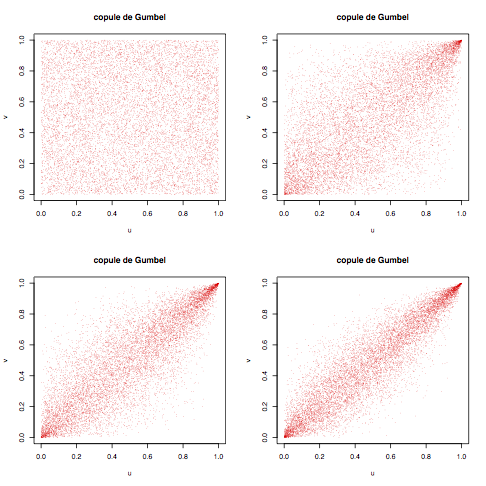
\includegraphics[scale=0.6]{img/simulation1234.png}
% \caption{Trac\'es de couples $(u,v)$ de copule de Gumbel}
% \label{simulation1234}
% \end{center}
% \end {figure}
% 
% \clearpage

\section{Estimation et impl\'ementation}
Dans un premier temps, nous rappellons les m\'ethodes d'estimation pour calibrer une copule.
Ensuite, nous pr\'esentons notre package \soft{R} intitul\'e \pkg{gumbel} impl\'ementant tous les outils
n\'ecessaires \`a la copule de Gumbel.


\subsection{Les m\'ethodes de calibrage}
Tout comme les copules archim\'ediennes de Clayton et de Frank, la copule de Gumbel pr\'esente l'avantage d'avoir un seul param\`etre \`a calibrer.
Nous faisons un bref rappel des m\'ethodes d'estimation sp\'ecifiques aux copules.

\subsubsection{M\'ethode des moments}
Cette m\'ethode consiste \`a estimer les param\`etres $\theta$ des lois marginales et le param\`etre $\alpha$ de la copule par la m\'ethode des moments i.e.
\begin{enumerate}
\item r\'esoudre le syst\`eme \`a $d$ \'equations et $d$ inconnues
$$
\left\{ \begin{array}{c}
\overline X_n = f(\theta_1,\dots,\theta_d)\\
S_n^2 = g(\theta_1,\dots,\theta_d)\\
\mu_{3,n} = h(\theta_1,\dots,\theta_d)\\
\vdots\\
\end{array}
\right. ,
$$
o\`u $d$ d\'esigne la dimension de $\theta$, $f$, $g$ et $h$ sont les expressions des moments (ordinaires) d'ordre 1, 2 et 3 en fonction du param\`etre $\theta$.
r\'epeter cette \'etape pour toutes les marginales.
\item inverser le tau de Kendall ou le rho de Spearman pour obtenir le param\`etre $\alpha$ de la copule.
\end{enumerate}

Pour des marginales exponentielles $\mathcal E(\lambda)$ et une copule de Gumbel, on trouve
$$
\hat \lambda_n = \frac{1}{\overline X_n}
\textrm{~~et~~}
\hat \alpha_n = \frac{1}{1-\tau_n},
$$
o\`u $\tau_n$ d\'esigne le tau de Kendall empirique. 


\subsubsection{Maximum de vraisemblance exact}
Dans le cas o\`u la densit\'e de la copule existe, on peut utiliser les estimateurs de maximum de vraisemblance. Pour simplifier, on suppose qu'on utilise une copule
bivari\'ee $C_\alpha$, ayant une densit\'e et que les lois des marginales poss\`edent des densit\'es. On note $\theta_1$ et $\theta_2$ les param\`etres des lois 
marginales. La log vraisemblance s'\'ecrit :
\begin{multline*}
\ln \mathcal L(\alpha, \theta_1, \theta_2, x_1,\dots, x_n, y_1,\dots, y_n) = \sum_{i=1}^n \ln\left( c \left( F_1(x_i,\theta_1), F_2(y_i,\theta_2),\alpha \right)\right) \\
+\sum_{i=1}^n \ln\left(f_1(x_i,\theta_1) \right) + \sum_{i=1}^n \ln\left(f_2(y_i,\theta_2) \right).
\end{multline*}
Bien souvent, il n'existe pas d'expressions explicites des estimateurs maximisant $\ln \mathcal L$, et on r\'ealise donc une maximisation num\'erique.

\subsubsection{Inf\'erence sur les marginales}
Toujours dans l'hypoth\`ese o\`u la copule a une densit\'e, on peut m\'elanger les deux premi\`eres approches, en estimant d'abord les param\`etres
des lois marginales, puis en estimant le param\`etre de la copule. Cela consiste \`a :
\begin{enumerate}
\item estimer les param\`etres $\theta_1$ et $\theta_2$ par maximum de vraisemblance
\item construire les pseudo donn\'ees $\forall 1\leq i \leq n, ~u_i = F_1(x_i, \hat \theta_1)$ et $v_i = F_2(y_i, \hat \theta_2)$
\item estimer le param\`etre $\alpha$ en maximisant la log-vraisemblance 
$$\ln \mathcal L(\alpha, u_1,\dots, u_n, v_1,\dots, v_n) = \sum_{i=1}^n \ln\left( c \left( u_i, v_i,\alpha \right)\right).$$
\end{enumerate}
Cette m\'ethode pr\'esente l'avantage d'utiliser les estimateurs ``classiques'' de maximum vraisemblance des marginales.

\subsubsection{Maximum de vraisemblance canonique}
C'est une m\'ethode semi-param\'etrique, qui se base sur la m\'ethode pr\'ec\'edente :
\begin{enumerate}
\item calculer les fonctions de r\'epartition empirique $F_{1,n}$ et $F_{2,n}$
\item construire les pseudo donn\'ees $\forall 1\leq i \leq n, ~u_i = F_{1,n}(x_i)$ et $v_i = F_{2,n}(y_i)$
\item estimer le param\`etre $\alpha$ en maximisant la log-vraisemblance 
$$\ln \mathcal L(\alpha, u_1,\dots, u_n, v_1,\dots, v_n) = \sum_{i=1}^n \ln\left( c \left( u_i, v_i,\alpha \right)\right).$$
\end{enumerate}

\subsection{Le package \soft{R} \pkg{gumbel}}
Nous avons r\'ealis\'e un package \soft{R} pour la copule de Gumbel. Les package \soft{R} pr\'esentent le gros avantage
de fournir rapidement du code document\'e, et donc r\'eutilisable par quelqu'un d'autres que ses concepteurs.


Notre package \pkg{gumbel}  fournit la fonction de r\'epartition : \code{pgumbel} (valable en dimension $n$),
la densit\'e : \code{dgumbel} (valable pour $n\leq 3$) et un g\'en\'erateur al\'eatoire : \code{rgumbel} 
(valable en dimension $n$ quelconque).

De plus, nous avons impl\'ement\'e les 4 m\'ethodes d'estimation pr\'esent\'ees ci dessus:
\begin{itemize}
\item la m\'ethode des moments (``Moment-Based Estimation'') : \code{gumbel.MBE},
\item le maximum de vraisemblance exacte (``Exact Maximum Likelihood'') : \code{gumbel.EML},
\item l'inf\'erence sur les marginales (``Inference For Margins'') : \code{gumbel.IFM},
\item le maximum de vraisemblance canonique (``Canonical Maximum Likelihood'') : \code{gumbel.CML}.
\end{itemize}
L'aide (en anglais) pour les diff\'erentes fonctions s'obtient avec la commande \code{help} le nom de la fonction
ou plus simplement \code{help(gumbel)} apr\`es avoir charg\'e le package \`a l'aide \code{library("gumbel")}.
Dans cette aide figure les d\'etails sur l'utilisation des diff\'erentes fonctions ainsi que des exemples.

\section{Application aux couvertures de produits indiciels}
La copule de Gumbel a l'avantage de d\'ecrire les d\'ependances asym\'etriques, 
o\`u les coefficients de queue inf\'erieure et de queue sup\'erieure diff\`erent.
Elle poss\`ede la caract\'eristique de pouvoir repr\'esenter des risques dont la structure 
de d\'ependance est accentu\'ee sur la queue sup\'erieure. 
De mani\`ere g\'en\'erale, la copule de Gumbel est \`a ce titre particuli\`erement adapt\'ee 
en assurance et en finance pour \'etudier l'impact de la survenance d'\'ev\'enements de forte 
intensit\'e sur la d\'ependance entre branches d'assurance, actifs financiers ou indices.
Nous illustrons cette caract\'eristique avec l'application suivante sur la couverture d'un produit indiciel,
o\`u nous allons prendre en compte la d\'ependance entre stations m\'et\'eorologiques pour
la construction d'un indice.



\subsection{Pr\'esentation}
Nous avons utilis\'e la copule de Gumbel pour valoriser les couvertures indicielles cat[as-trophe]. Ces contrats sont des d\'eriv\'es
climatiques adapt\'es \`a la r\'eassurance d'\'ev\`enement catastrophe (tempÍte, vague de froid,\dots) bas\'e sur un indice climatique
(force du vent, temp\'erature,\dots). Cette application num\'erique est bas\'ee sur l'article \cite{benfield}.

L'indice climatique doit refl\'eter au mieux les caract\'erisques des montants des sinistres associ\'es au risque m\'et\'eo pour diminuer
le risque de base. En g\'en\'eral, on choisit un panier de $n$ stations (peu \'eloign\'ees des r\'egions assur\'ees) dans lesquelles on 
mesure la variable climatique $X_i(t)$ au cours de la p\'eriode $[t-1,t]$. Ensuite, l'indice journalier d'une station $i$ est construit
par $I_i(t) = \min(L_i-K_i, X_i(t) - K_i)$ o\`u $K_i$ et $L_i$ sont le seuil et la limite par station. Sur une p\'eriode $T$, l'indice d'une station 
est donc d\'efini par $S_i(T) = \sum_{t=1}^T I_i(t)$ et l'indice cumul\'e par $S_T =  \sum_{i=1}^n p_i S_i(T)$ pour une pond\'eration 
$p_1, \dots, p_n$. Enfin le flux engendr\'e par la couverture indicielle est celui d'un call spread : $$C_T = N \times 
\min\left(L-K, \left(S_T-K\right)_+\right),$$
o\`u $K$ et $L$ sont la franchise et la limite du contrat, et $N$ le montant nominal.

Pour notre exemple, on traite les risque ``temp\^ete'' en Rh\^one Alpes. $X_i(t)$ d\'esigne donc la force maximale du vent (en m/s) par jour.
Nous avons choisi deux stations Saint Martin en Haut (variable $X$) et Echirolles (variable $Y$) avec les seuils respectifs $10$ et $9$, et les limites $16$ et $15$\footnote{les seuils sont volontairement bas.}. On prend $T=600$ jours, $N=1$, $K=50$ et $L=200$.

\subsection{Calibration}
Il faut calibrer la copule de Gumbel sur nos donn\'ees recueillies sur les sites internet \code{www.meteoisere.com/Vantage}  et
\code{hautsdulyonnais.free.fr/} entre ao\^ut 2005 et avril 2007. Pour ce faire, un choix de marginales s'impose. Des marginales
exponentielles se r\'ev\'elant totalement d\'esastreux\footnote{le test de Kolmogorov Smirnov rejette outrageusement
l'hypoth\`ese que les donn\'ees suivent une loi exponentielle, tandis que le trac\'e de la fonction de r\'epartition empirique
et de la fonction de r\'epartition de l'exponentielle r\'ev\`ele tr\`es clairement que l'hypoth\`ese exponentielle est 
impossible.}, nous avons choisi des marginales gamma dont les param\`etres de forme 
et de taux sont not\'es $\alpha_X$, $\lambda_X$ pour Saint Martin en Haut
et $\alpha_Y$, $\lambda_Y$ pour Echirolles. On pose $\alpha_{cop}$ le param\`etre de la copule de Gumbel. 
Le tableau \ref{estim} infra r\'ecapitule nos r\'esultats d'estimation :
\begin{table}[!htb]
\center
\begin{tabular}{lccccc}
\hline
M\'ethodes & MBE & EML & IFM & CML & moyenne\\
\hline
$\alpha_X$ & 4,885 & 4,954 & 4,833 & - & 4,891\\
\hline
$\lambda_X$ & 0,747 & 0,754 & 0,739 & - & 0,746\\
\hline
$\alpha_Y$ & 6,810 & 6,824 & 7,161 & - & 6,932\\
\hline
$\lambda_Y$ & 1,121 & 1,116 & 1,178 & - & 1,139\\
\hline
$\alpha_{cop}$ & 1,533 & 1,461 & 1,448 & 1,474 & 1,479\\
\hline
\end {tabular}
\caption{Estimations des param\`etres}
\label{estim}
\end{table}

Pour la suite, nous choisissons les moyennes des estimations comme valeur de nos param\`etres.
Le bon ajustement des marginales se voit sur les graphes de la figure \ref{marginale}, o\`u l'on voit
que les fonctions de r\'epartitions calibr\'ees (i.e. gamma avec les param\`etres supra) s'ajustent
bien sur les fonctions de r\'epartitions empiriques.
% \begin{figure}[!htb]
% \begin{center}
% 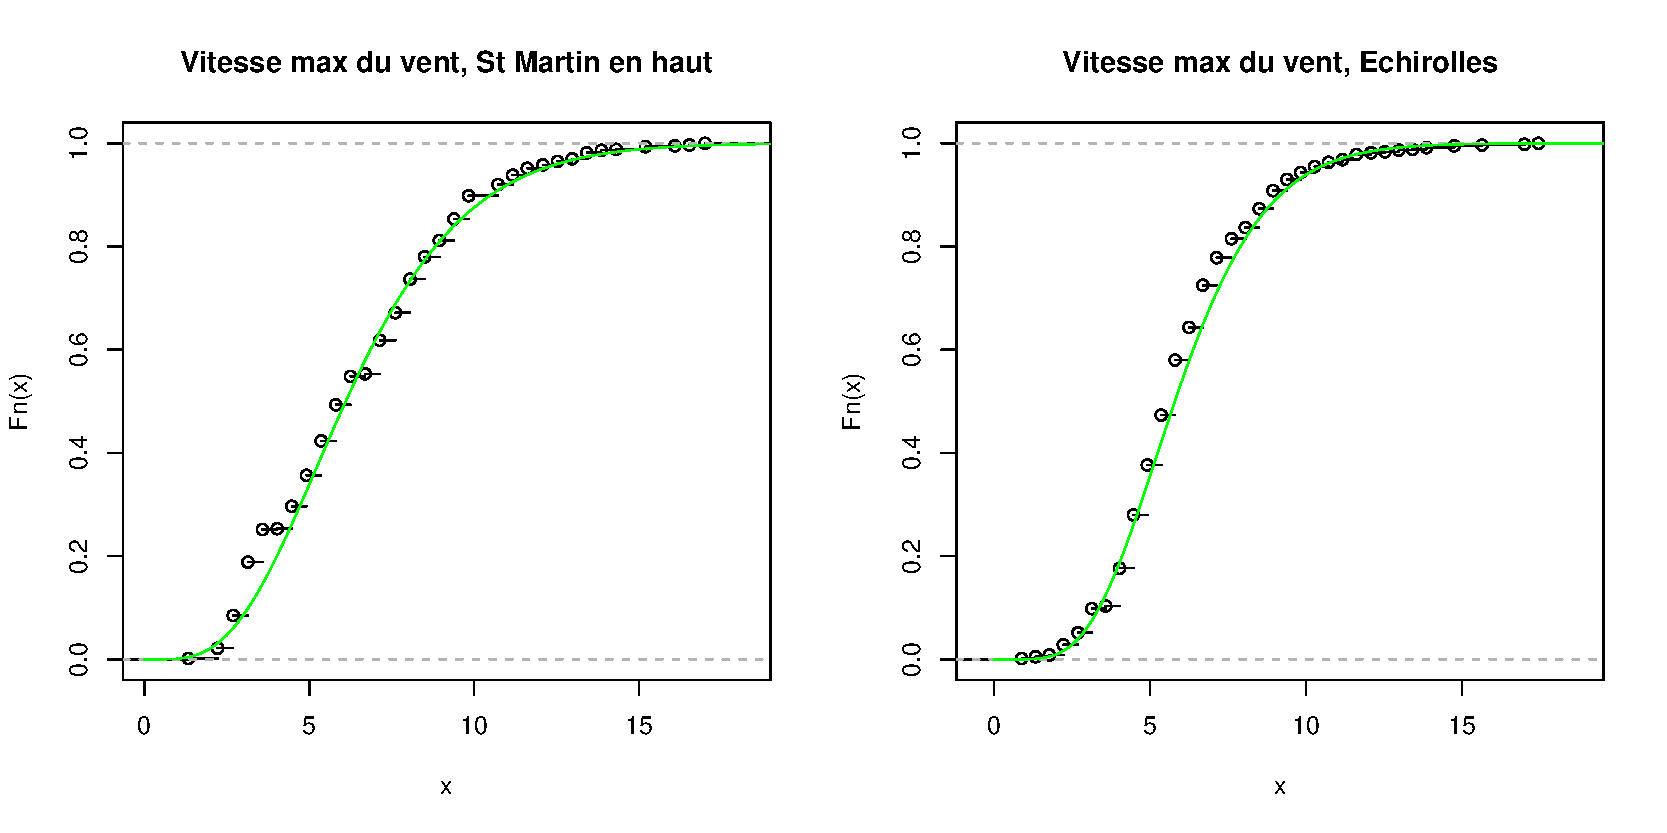
\includegraphics[scale=0.56]{img/marginale.pdf}
% \caption{Fonctions de r\'epartitions empiriques (en noir) et calibr\'ees (en vert)}
% \label{marginale}
% \end{center}
% \end {figure}

La bonne ad\'equation de la copule de Gumbel aux vitesses de vent maximales est confirm\'e
par le trac\'e d'un qqplot empirique (cf. figure \ref{qqplot}). Les nuages semblent \'equivalents.
A priori, la copule de Gumbel est faite pour mod\'eliser une d\'ependance des ``extr\^emes'', puisqu'elle
est asym\'etrique.
% \begin{figure}[!htb]
% \begin{center}
% 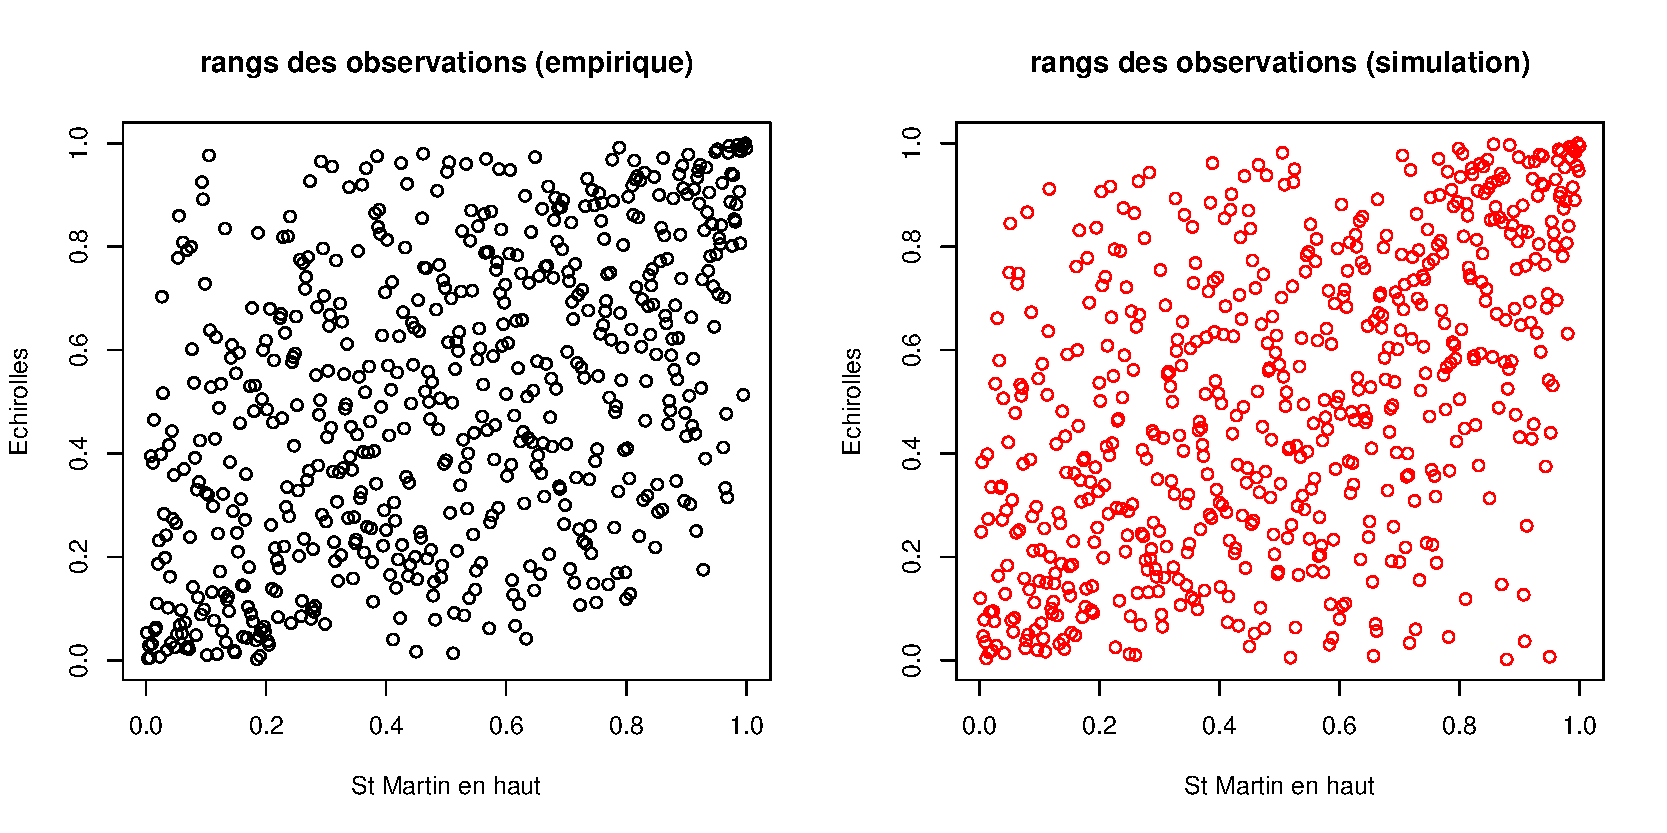
\includegraphics[scale=0.56]{img/qqplot.pdf}
% \caption{qqplot empirique vs simul\'e}
% \label{qqplot}
% \end{center}
% \end {figure}

\subsection{Evaluation du payoff}
Maintenant que l'on a calibr\'e notre copule (et les marginales), on va estimer le payoff $C_T$ par une m\'ethode
de Monte Carlo. Nous avons r\'ealis\'e 10000 simulations de p\'eriode de 600 jours pour nos deux stations. Nous obtenons
les r\'esultats infra (tableau \ref{payoff}). On constate que m\^eme si la d\'ependance fait diminuer en moyenne le payoff,
l'\'ecart type et le quantile \`a $75\%$ augmentent. Tout semble laisser penser que la d\'ependance augmente
la queue de distribution.
\begin{table}[!htb]
\center
\begin{tabular}{lccccc}
\hline
$\alpha_{cop}$ & 1 & 1,25 & 1,479 (valeur estim\'ee) & 1,75 & 2\\
\hline
moyenne & 79,21 & 79,14 & 79,11 & 78,93 & 78,95 \\
\hline
\'ecart-type & 13,96 & 16,27 & 16,99 & 17,84 & 18,17\\
\hline
$VaR_{75\%}$ & 88,69 & 89,94 & 90,26 & 90,68 & 91,03\\
\hline
$VaR_{90\%}$ & 97,24 & 100,13 & 101,23 & 102,37 & 102,72\\
\hline
\end{tabular}
\caption{Statistiques des payoff $C_T$ simul\'es}
\label{payoff}
\end{table}


Enfin, nous avons trac\'e les histogrammes (cf. figure \ref{histogramme}) \`a pas fixe et \`a mÍme effectif du payoff correspondant
\`a nos donn\'ees ($\alpha_{cop}= 1,479 $). Nous pouvons constater que la distribution
des sinistres est l\'eg\`erement asym\'etrique, surtout autour de sa moyenne. Par ailleurs, nous avons ajout\'e
l'estimation de la densit\'e par la m\'ethode du noyau d'Epanechnikov. Maintenant, il ne reste plus qu'\`a choisir
un principe de primes et calculer le prix de ce produit de couverture indiciel virtuel.
% \begin{figure}[!htb]
% \begin{center}
% 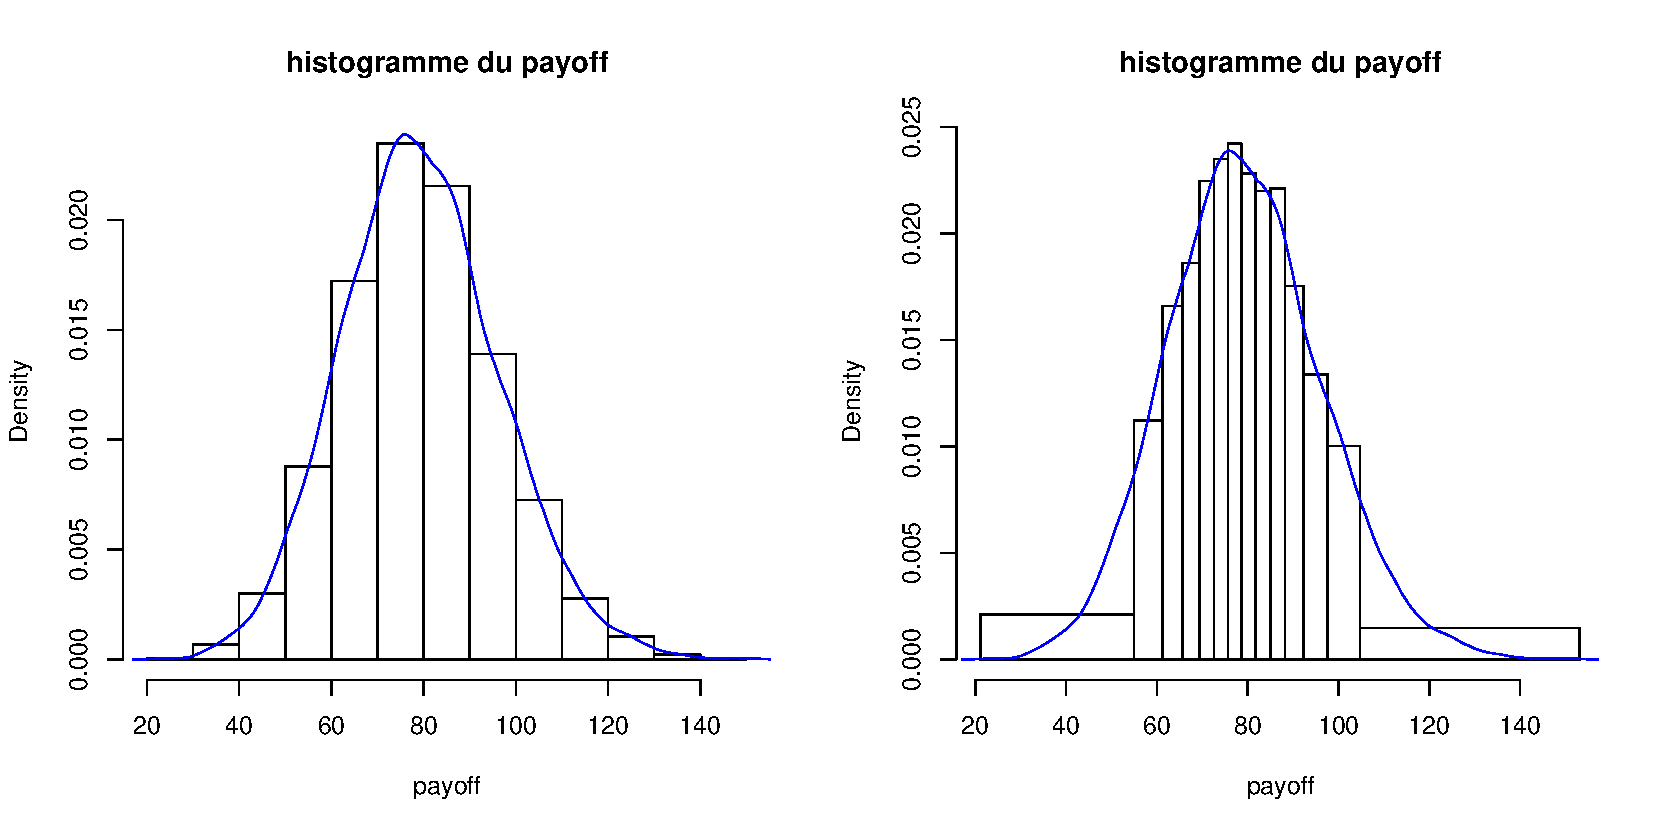
\includegraphics[scale=0.56]{img/histogramme.pdf}
% \caption{Histogrammes \`a pas fixe et \`a m\^eme effectif}
% \label{histogramme}
% \end{center}
% \end {figure}




%la bibliographie
\addcontentsline{toc}{section}{Bibliographie}
\bibliographystyle{agsm}  
\bibliography{gumbel}    


%annexes
\section*{Annexes}
\addcontentsline{toc}{section}{Annexes}
\appendix
\begin{small}


\section{Densit\'e de la copule de Gumbel}
\label{densiteDemo}
On a 
\begin{center}
\fbox{$\forall u, v \in ]0,1[^2, c_\alpha(u,v)=C_\alpha(u,v) \frac{\phi_{\alpha-1}(u)\phi_{\alpha-1}(v)}{uv}   \left[ \phi_{\alpha}(u)+\phi_{\alpha}(u)  \right]^{\frac{1}{\alpha}-2}\left[ \alpha-1+\left( \phi_{\alpha}(u)+\phi_{\alpha}(u)\right)^{\frac{1}{\alpha}} \right] $}
\end{center}


L'expression supra de la densit\'e n'est pas valable sur les bords du pav\'e $[0,1]\times [0,1]$. En effet, si on cherche \`a calculer
la d\'eriv\'ee seconde crois\'ee $\frac{\partial^2 C}{\partial u \partial v}\footnote{Pour simplifier, on omet l'indice $\alpha$.}$ en des points du bord, alors on constate qu'elle n'est pas d\'efinie.
Dans un premier, on calcule $\frac{\partial C}{\partial u }(0,v)$ : 
\begin{eqnarray*}
\frac{C(0+h,v)-C(0,v)}{h-0} &= &\frac{C(h,v)}{h}
= e^{-\ln h}e^{-\left[ (-\ln h)^\alpha+(-\ln v)^\alpha  \right]^{\frac{1}{\alpha}}} 
= e^{-\ln h }e^{+\ln h \left[ 1+(\frac{\ln v}{\ln h})^\alpha  \right]^{\frac{1}{\alpha}}} \\
&=& e^{\ln h\left[ \left[1+(\frac{\ln v}{\ln h})^\alpha  \right]^{\frac{1}{\alpha}} -1\right] } 
\underset{h\rightarrow 0}{\longrightarrow} 1,
\end{eqnarray*}
puisque en r\'ealisant un d\'eveloppement limit\'e (DL) de l'exposant, on a: 
$$\left[1+ \left(\frac{\ln v}{\ln h} \right)^\alpha  \right]^{\frac{1}{\alpha}} = 1+\frac{1}{\alpha} \left(\frac{\ln v}{\ln h} \right)^\alpha+O\left(\left(\frac{\ln v}{\ln h} \right)^\alpha\right).$$
Donc, on a
$$
\frac{\partial C}{\partial u }(0,v) = 1 \textrm{~et par sym\'etrie~} \frac{\partial C}{\partial v }(u,0) = 1.
$$
De m\^eme, on trouve
$$
\frac{\partial C}{\partial u }(0,0) = 0 \textrm{~et par sym\'etrie~} \frac{\partial C}{\partial v }(0,0) = 0.
$$
puisque $C(0+h,0)=C(0,0)=0$.
Enfin, on aboutit \`a la non existence de $\frac{\partial^2 C}{\partial u \partial v}(0,0)$, par
$$
\frac{\frac{\partial C}{\partial u }(0,h)-\frac{\partial C}{\partial u }(0,0)}{h-0} =\frac{1}{h}\underset{h\rightarrow 0}{\longrightarrow} +\infty
$$
En se servant des calculs pr\'ec\'edents, on trouve que $\forall 0<u,v<1,~\frac{\partial^2 C}{\partial u \partial v}(0,v) = \frac{\partial^2 C}{\partial u \partial v}(u,0)=0$


En appliquant le m\^eme raisonnement (i.e. avec un DL), on trouve que 
$$
\frac{\partial C}{\partial u }(1,v) \stackrel{\triangle}{=} \underset{h\rightarrow 0}{\lim} \frac{C(1,v)-C(1-h,v)}{h} = 0
$$
et
$$
\frac{\partial C}{\partial u }(1,1) \stackrel{\triangle}{=} \underset{h\rightarrow 0}{\lim} \frac{C(1,1)-C(1-h,1)}{h} = 1
$$
D'o\`u, la non existence de  $\frac{\partial^2 C}{\partial u \partial v}(1,1)$ par
$$
\frac{\frac{\partial C}{\partial u }(1,1)-\frac{\partial C}{\partial u }(1,1-h)}{1-(1-h)} =\frac{1}{h}\underset{h\rightarrow 0}{\longrightarrow} +\infty
$$
Enfin, on a aussi, $\forall 0<u,v<1,~\frac{\partial^2 C}{\partial u \partial v}(1,v) = \frac{\partial^2 C}{\partial u \partial v}(u,1)=0$.

\section{Valeur particuli\`ere de $\alpha$}
\label{parametreDemo}
Pour $\alpha=1$, on a 
$$
C_1(u,v) = C_\alpha\left(u,v\right)=\exp\left[-\left(\left(-\ln u\right)^1+\left(-\ln v\right)^1\right)^1\right] = uv
$$
Autrement dit, $C_1$ est la copule d'ind\'ependance.

De plus, si on suppose $u\leq v$, alors
$$
C_\alpha(u,v) = \exp\left[-\left(\left(-\ln u\right)^\alpha+\left(-\ln v\right)^\alpha\right)^{\frac{1}{\alpha}}\right] 
      =  \exp \left[  \ln u \left(\left(\frac{\ln v}{\ln u}\right)^\alpha+1\right)^{\frac{1}{\alpha}}\right] 
      \underset{\alpha\rightarrow +\infty}{\longrightarrow} v
$$
Ainsi $C_\infty = C^+$ la copule de la borne sup\'erieure de Fr\'echet, i.e. la copule comonotone.

Il est important de noter que quelques soit $\alpha$, la copule de Gumbel permet de mod\'eliser seulement des d\'ependances positives.


\section{D\'ependance des extr\^emes}
\label{extreme}
Par un r\'esultat de \cite{nelsen}, on a que 
$$\lambda_U =2-\underset{t\rightarrow0^+}{\lim} \frac{1-\phi^{-1}(2t) }{1-\phi^{-1}(t)} \txtm{et}
\lambda_L = \underset{t\rightarrow +\infty}{\lim} \frac{\phi^{-1}(2t) }{\phi^{-1}(t)}.
$$
Pour notre copule de Gumbel, on a 
$$
\lambda_U =2-\underset{t\rightarrow0^+}{\lim} \frac{1- e^{-(2t)^\frac{1}{\alpha}} }{1- e^{-t^\frac{1}{\alpha}} }
= 2- \frac{1- \left(1-(2t)^\frac{1}{\alpha}  +O\left(t^\frac{1}{\alpha}\right)\right) }{1- \left(1-t^\frac{1}{\alpha} +O\left(t^\frac{1}{\alpha}\right)\right) }
= 2- \frac{ (2t)^\frac{1}{\alpha}  +O\left(t^\frac{1}{\alpha}\right) }{ t^\frac{1}{\alpha} +O\left(t^\frac{1}{\alpha}\right) }
\underset{t\rightarrow0^+}{\longrightarrow} 2- 2^\frac{1}{\alpha},
$$
et 
$$
\lambda_L = \underset{t\rightarrow +\infty}{\lim} \frac{ e^{-(2t)^\frac{1}{\alpha}}  }{ e^{-t^\frac{1}{\alpha}} }
= \underset{t\rightarrow +\infty}{\lim} e^{ - (2^\frac{1}{\alpha}-1)t^\frac{1}{\alpha} } =0.
$$



La copule de Gumbel v\'erifie la propri\'et\'e de max-stabilit\'e :
\begin{align*}
C_\alpha\left(u^{1/r},v^{1/r}\right)^r &= \left[ \exp\left[-\left(\left(-\ln u^{1/r}\right)^\alpha + \left(-\ln v^{1/r}\right)^\alpha\right)^\frac{1}{\alpha}\right] \right]^r 
                                       = \exp\left[ -r\left(\left(-\frac{1}{r}\ln u\right)^\alpha + \left(-\frac{1}{r}\ln v\right)^\alpha\right)^\frac{1}{\alpha} \right] \\
                                      & = \exp\left[ -\left(\left(-\ln u\right)^\alpha + \left(-\ln v\right)^\alpha\right)^\frac{1}{\alpha} \right] = C_\alpha(u,v)
\end{align*}

\end{small}
\end{document}
